% !TEX root = thesis.tex

% Front cover
% \includepdf{cover-front.pdf}

% Half-title
\maketitle


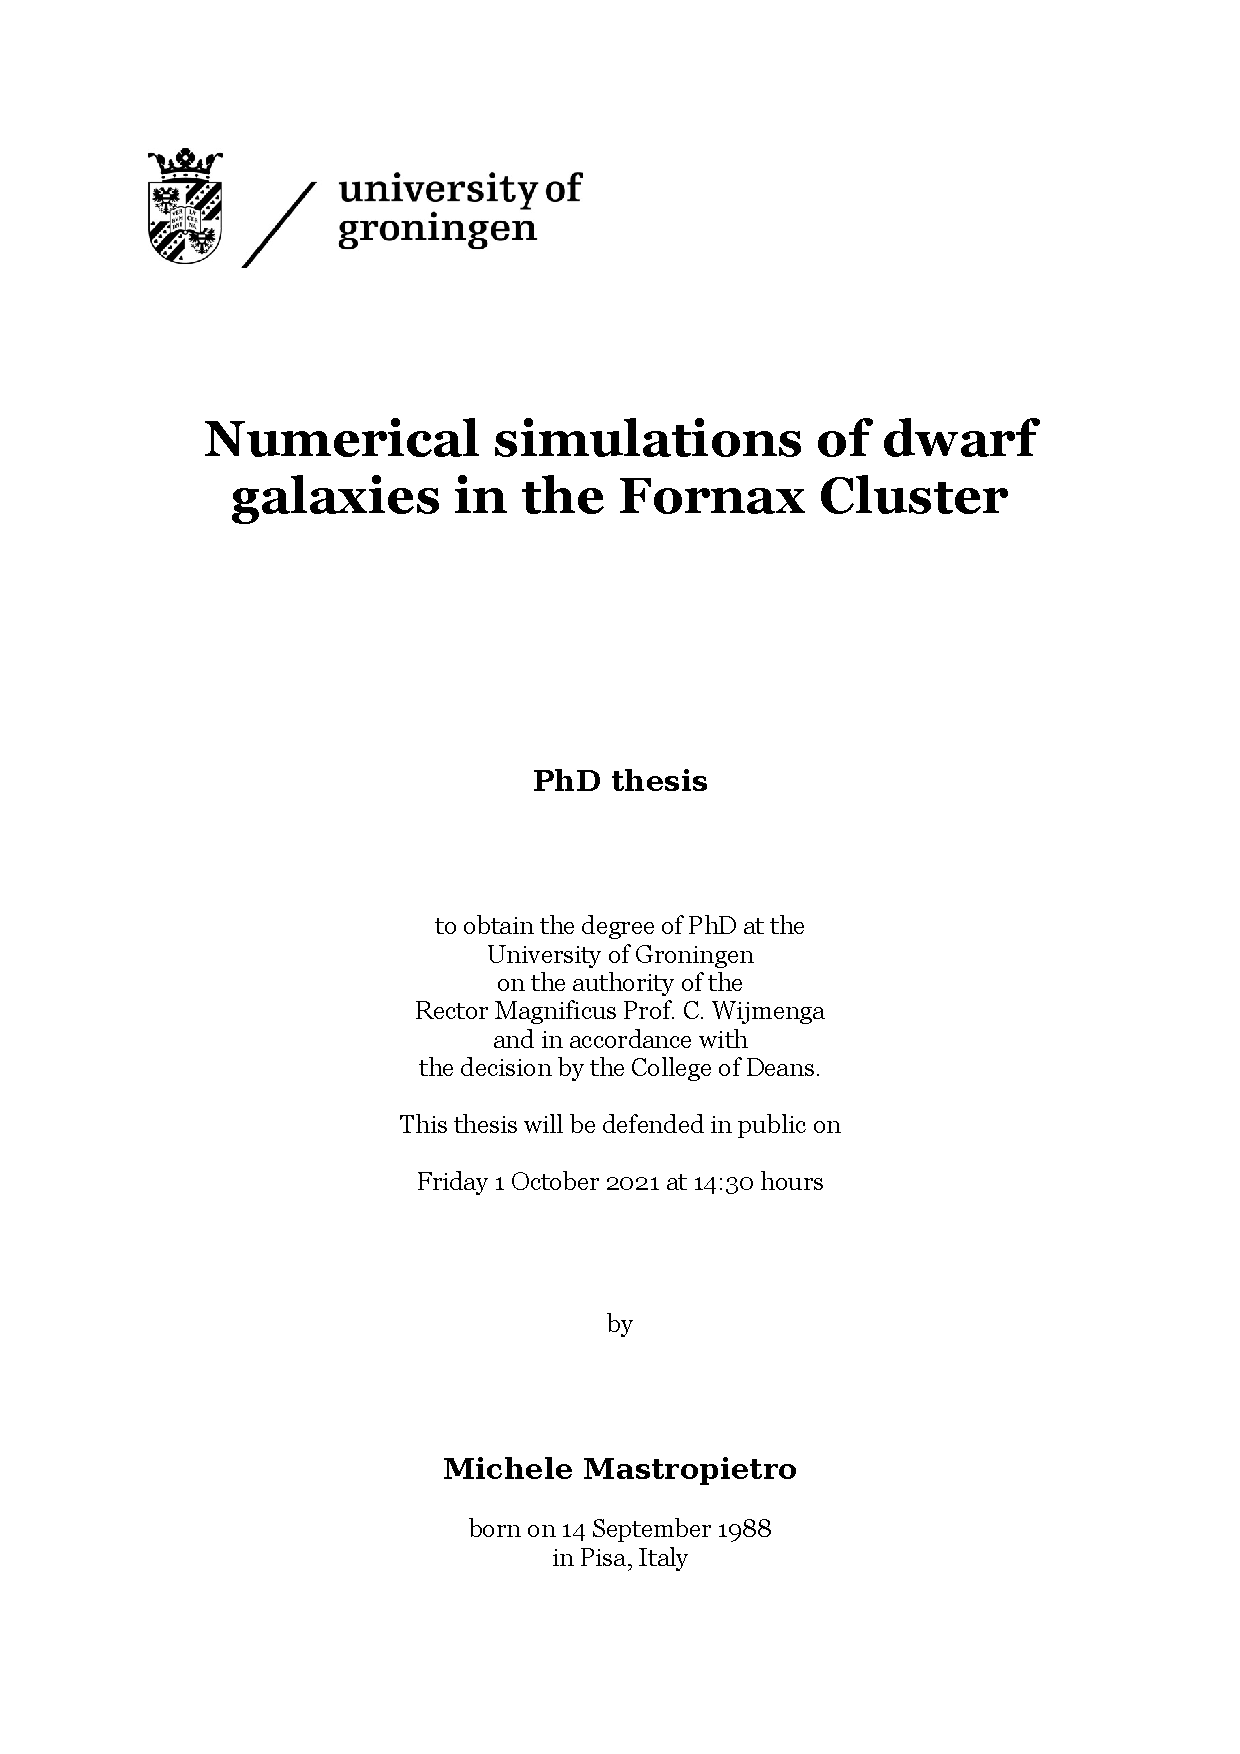
\includepdf[pages=-]{title_page.pdf}


\begin{comment}
% Official title
\begin{titlepage}
\null%
\label{thesis:title}
\vspace{3em}%
\pdfbookmark[1]{Title}{thesis:title}
\begin{center}

%% Skip space as in half-title
\vspace*{4\baselineskip}

%% Print the title.
\makeatletter
{\huge\@title}
\makeatother
\vfill

{\Large Proefschrift}

\medskip

{voorgedragen tot het behalen van \\
de graad van
Doctor in de Fysica en Sterrenkunde}


\medskip

door

\medskip

\makeatletter
{\Large \@author}
\makeatother

\medskip

aan de\\
{\large Universiteit Gent}\\
en aan de\\
{\large Rijksuniversiteit Groningen}\\
% Graduate School of Science and Engineering\\

\end{center}
\end{titlepage}





% Official verso
\clearpage
\thispagestyle{empty}
\null%
\label{thesis:committee}
\vfill
\pdfbookmark[1]{Doctoral committee}{thesis:committee}

% \noindent Members of the examination board:

\medskip\noindent
\begin{tabular}{@{}lll@{}}{Promotors:}\\\\
  \quad{}Prof.\ dr. Sven De Rijcke & Ghent University & (promotor)\\
  \quad{}Prof.\ dr. Michael\ Biehl & University of Groningen & (promotor)\\
  \quad{}Prof.\ dr. Reynier\ Peletier & University of Groningen & (promotor)\\
\\\\
\multicolumn{2}{@{}l@{}}{Composition of the Joint Evaluation Committee:} \\
\\
%   \quad{}Prof.\ dr.\  & chairperson \\
   \quad{}Prof.\ dr.\ Frazer Pearce & University of Nottingham\\
   \quad{}Prof.\ dr.\ Arjen van der Wel & Ghent University \\
   \quad{}Prof.\ dr.\ John McKean & University of Groningen \\
   \quad{}Prof.\ dr.\ Hugues Talbot & Université Paris-Saclay\\
\medskip\noindent
%   \quad{}Dr.\ & University of Groningen\\
% \\
% \multicolumn{2}{@{}l@{}}{Independent members:} \\
% \\
%   \quad{}Prof.\ dr.\ & University of Technology \\
%   \quad{}Prof.\ dr.\ & University \\
%   \quad{}Dr.\& University \\
% \\
% \multicolumn{2}{@{}l@{}}{Other member:} \\
% \\
%   \quad{}Dr.\ & ...\\
\end{tabular}
\end{comment}



% Copyright page
\clearpage
\thispagestyle{empty}
\null%
\label{thesis:colophon}
\vfill
\pdfbookmark[1]{Colophon}{thesis:colophon}
\noindent Written in 2021 by {\makeatletter{\@author}\makeatother}.\\
\textbf{Copyright}~\cczero{} The template for the layout of this thesis was inspired by my colleague Sam Verstocken who used the template of the dissertation of \href{ken.mx}{Ken Arroyo Ohori},
which was released into the public domain using the Creative~Commons~\cczero{}~code.
To view a copy of the \cczero{}~code, visit:\\\url{http://creativecommons.org/publicdomain/zero/1.0/}\\
\textbf{Colophon}
% This thesis was typeset with \XeTeX, Version 3.14159265-2.6-0.99998 (TeX Live 2017/Debian) using the \mbox{{\fanciestfont{}Feijoa}}, \texttt{GT Pressura} and $\mathrm{Asana\ Math}$ typefaces.
Most of the figures were created using \href{http://ipe.otfried.org/}{Ipe} (Copyright © 1993–2020 Otfried Cheong).
The source code of this thesis is available at: \\
\url{https://github.com/elehcim/phd-thesis}\\
\textbf{Cover}
...\\[2ex]
This research was funded by the European Union's Horizon 2020 research and innovation programme under the Marie Sk\l odowska-Curie
% Skłodowska-Curie
grant agreement N.~721463 to the \href{www.astro.rug.nl/~sundial}{SUNDIAL ITN network}.
\begin{figure*}[bh!]
  \centering
  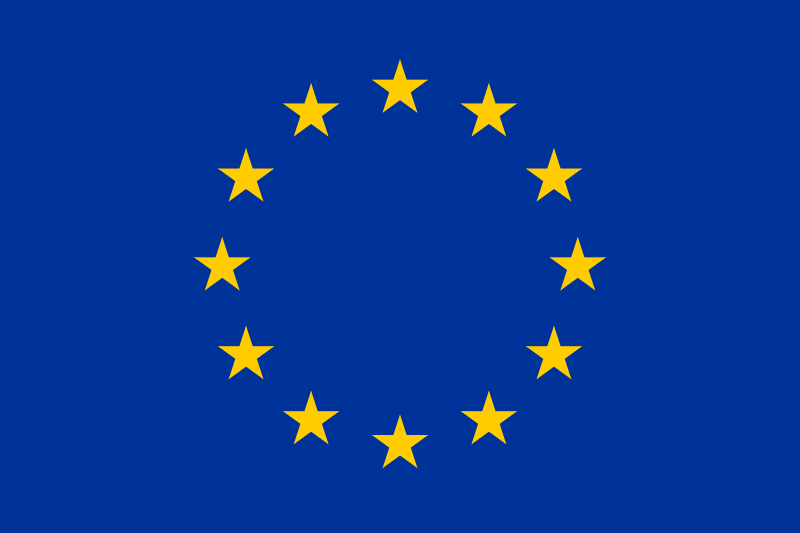
\includegraphics[width=0.2\textwidth]{EUflag}
\end{figure*}

% Aknowledgements page
\clearpage
\thispagestyle{empty}
\null%
\label{thesis:acknowledgements}
  \begin{center}
    {\Large \textbf{Acknowledgements}}\\
  \end{center}
\pdfbookmark[1]{Acknowledgements}{thesis:acknowledgements}
I'd like to thank first of all my professor Sven De Rijcke who first believed in me doing a PhD from the first email in February 2017. I thank you Sven for showing me what science is, how can it be difficult but also how it is a gym to train in deep honesty. I've learned from you how to cope with difficulties (especially in these pandemic times) in a very mature and ironic way.
Thank you also for being a mirror for me in our meetings, and always pushing me up even in my down moments.

The SUNDIAL project has been one of the nicest group of people I've ever met. I'll never forget the high quality of people, their professionalism, attention and kindness for all of us.
Thank you Reynier, our PI, supervisor of all of us, always available to investigate new ideas despite the many obligations and meetings you had to attend: thanks for inspiring us in how you live astronomy and education of young scientists as a calling.
%Thank you Johan, my external mentor, for the interest you showed in my, for being kind and firm showing me how to clearly express.
The collaboration among us ESRs has often ended up in very good friendship, and I'll always remember the many memorable moments we lived together (in Naples, La Palma, Ghent...).

I thank my fellow astronomer colleagues at S9, the ones who are there, the ones who left during these years and the ones who just arrived. I've learned so much from you academically and how to work happily and work.
The Belgian ``old guard": Maarten, Seba, Wouter, Sam, Marjorie, Dries, Robbert, Bert; thank you for welcoming me. Thanks to Ana and Goran, Caroline, Aaron.
You have been so nice towards me, that's been an honour to work in the same place as you.
Thank you dear office mates: Caroline, Sara and Anand for the discussions and the nice coffe and fruit breacks. Caro, thank you for all the support, deep sharing and friendship.
Thank you for the many parties and dinners and the initiation rites invented from nothing.
I also thank the precious group of the Maxwell Demons: nice people to play minifootball and with real team spirit.
Thank you Shivangee, office mate, companion of the Sundial advernture, and of the life in Gent. Thank you for your constant unbroken positive attitude always: in happy high moments as well as the low difficult times of PhD far from home.
Thank you Daniela and Andrea, young fellow of survival in in lockdown times: I had so many great moments with you.

Finally I thank Angelos, a real "Sam" for me, in the sense of the Lord of the Rings: so many times helping me and pulling me out of my down moments with frank conversations (is it a perk of living in Frank Baurstraat? ;P ), sharing deep insights of life and being the fuel of many parties and gatherings, always with a lot of attention to everyone.

Many thanks go to the community of the Apostoline helping me in many ways in these years.
Thank you Pinco for constant example of free giving.

I thank my family: mamma e babbo, for your constant, positive, caring attitude towards me. Mi stupisco spesso di come siate davvero i genitori che vorrei avere, in tutti questi anni.
Anto for the cristalline confrontation and the sensitivity, Fra for the innumerable funny stories and deep insights. Nonna Lida per esserci ed essere una roccia salda per tutti, always.

% Summary page
\clearpage
\thispagestyle{empty}
\null%
\label{thesis:Summary}
\begin{center}
  {\Large \textbf{Summary}}\\
\end{center}
\pdfbookmark[1]{Summary}{thesis:Summary}

\clearpage
\thispagestyle{empty}
\null%
\begin{center}
  {\Large \textbf{Samenvatting}}\\
\end{center}

\clearpage
\thispagestyle{empty}
\null%
\begin{center}
  {\Large \textbf{Riassunto}}\\
\end{center}